%%%%%%%%%%%%%%%%%%%%%%%%%%%%%%%%%%%%%%%%%
% Beamer Presentation
% LaTeX Template
% Version 1.0 (10/11/12)
%
% This template has been downloaded from:
% http://www.LaTeXTemplates.com
%
% License:
% CC BY-NC-SA 3.0 (http://creativecommons.org/licenses/by-nc-sa/3.0/)
%
%%%%%%%%%%%%%%%%%%%%%%%%%%%%%%%%%%%%%%%%%

%----------------------------------------------------------------------------------------
%	PACKAGES AND THEMES
%----------------------------------------------------------------------------------------

\documentclass{beamer}

\mode<presentation> {

% The Beamer class comes with a number of default slide themes
% which change the colors and layouts of slides. Below this is a list
% of all the themes, uncomment each in turn to see what they look like.

%\usetheme{default}
%\usetheme{AnnArbor}
%\usetheme{Antibes}
%\usetheme{Bergen}
%\usetheme{Berkeley}
%\usetheme{Berlin}
%\usetheme{Boadilla}
%\usetheme{CambridgeUS}
%\usetheme{Copenhagen}
%\usetheme{Darmstadt}
%\usetheme{Dresden}
%\usetheme{Frankfurt}
%\usetheme{Goettingen}
%\usetheme{Hannover}
%\usetheme{Ilmenau}
%\usetheme{JuanLesPins}
%\usetheme{Luebeck}
\usetheme{Madrid}
%\usetheme{Malmoe}
%\usetheme{Marburg}
%\usetheme{Montpellier}
%\usetheme{PaloAlto}
%\usetheme{Pittsburgh}
%\usetheme{Rochester}
%\usetheme{Singapore}
%\usetheme{Szeged}
%\usetheme{Warsaw}

% As well as themes, the Beamer class has a number of color themes
% for any slide theme. Uncomment each of these in turn to see how it
% changes the colors of your current slide theme.

%\usecolortheme{albatross}
%\usecolortheme{beaver}
%\usecolortheme{beetle}
%\usecolortheme{crane}
%\usecolortheme{dolphin}
%\usecolortheme{dove}
%\usecolortheme{fly}
%\usecolortheme{lily}
%\usecolortheme{orchid}
%\usecolortheme{rose}
%\usecolortheme{seagull}
%\usecolortheme{seahorse}
%\usecolortheme{whale}
%\usecolortheme{wolverine}

%\setbeamertemplate{footline} % To remove the footer line in all slides uncomment this line
%\setbeamertemplate{footline}[page number] % To replace the footer line in all slides with a simple slide count uncomment this line

%\setbeamertemplate{navigation symbols}{} % To remove the navigation symbols from the bottom of all slides uncomment this line
}

\usepackage{graphicx} % Allows including images
\usepackage{booktabs} % Allows the use of \toprule, \midrule and \bottomrule in tables

\usepackage{tikz}
\usetikzlibrary{shapes.geometric,arrows}
\tikzset{
  basics/.style={minimum width=30mm, minimum height=7.5mm, text centered, draw=black},
  startstop/.style={rectangle, rounded corners, basics, fill=blue!10},
  io/.style={trapezium, trapezium left angle=70, trapezium right angle=110, basics, fill=blue!10},
  process/.style={rectangle, rounded corners, basics, fill=blue!10},
  decision/.style={ellipse,basics, fill=red!30},%green
  arrow/.style={thick,->,>=stealth},
}

%----------------------------------------------------------------------------------------
%	TITLE PAGE
%----------------------------------------------------------------------------------------

\title[GAL prediction]{Grasp-and-Lift EEG Detection } % The short title appears at the bottom of every slide, the full title is only on the title page

\author{Anirudhan J Rajagopalan, Michele Cer\'u} % Your name
\institute[UCLA] % Your institution as it will appear on the bottom of every slide, may be shorthand to save space
{
New York University \\ % Your institution for the title page
\medskip
\textit{ajr619@nyu.edu; mc3784@nyu.edu} % Your email address
}
\date{\today} % Date, can be changed to a custom date

\begin{document}

\begin{frame}
\titlepage % Print the title page as the first slide
\end{frame}



%\begin{frame}
%\frametitle{Overview} % Table of contents slide, comment this block out to remove it
%\tableofcontents % Throughout your presentation, if you choose to use \section{} and \subsection{} commands, these will automatically be printed on this slide as an overview of your presentation
%\end{frame}

%----------------------------------------------------------------------------------------
%	PRESENTATION SLIDES
%----------------------------------------------------------------------------------------

%------------------------------------------------
\section{First Section} % Sections can be created in order to organize your presentation into discrete blocks, all sections and subsections are automatically printed in the table of contents as an overview of the talk
%------------------------------------------------

\subsection{Subsection Example} % A subsection can be created just before a set of slides with a common theme to further break down your presentation into chunks

\begin{frame}
\frametitle{Project description}
Identify hand motions from EEG recordings
\begin{columns}[T]
\begin{column}{.5\textwidth}
\begin{itemize} 
\item Goal: classify hand motions from its EEG signal data.  
\item Purpose: Brain-Computer Interface prosthetic devices for restoring a patient's ability to perform basic daily tasks. 
\end{itemize}
\end{column}
\begin{column}{.5\textwidth}
\begin{center}
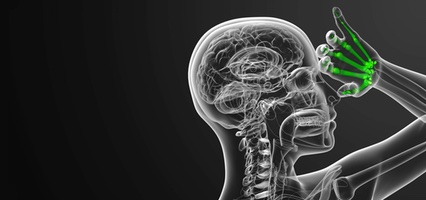
\includegraphics[height=1.0in]{front_page.png}
\end{center}
\end{column}
\end{columns}
  \end{frame}


\begin{frame}
\frametitle{Dataset}
32 EEG signals:
\begin{columns}[T]
\begin{column}{.5\textwidth}
\begin{center}
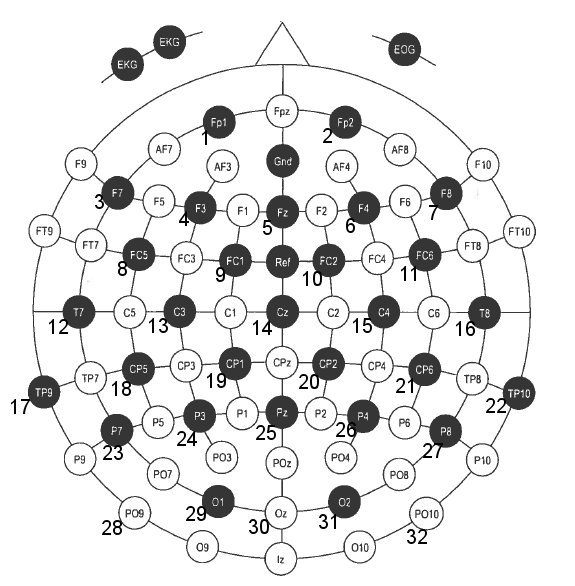
\includegraphics[height=2.0in]{EEG_Electrode_Numbering.jpg}
\end{center}
\end{column}
\begin{column}{.5\textwidth}
\begin{itemize} 
\item 30 Grasp And Lift series.
\item Training data set: 96 files
\item testing data set: 24 files
\item  Size: 1.5 Gb.
\item $17985850$ total number of samples
\item $\sim180k$ samples per subject
\item sampling rate: $ 500Hz$
\item Multi class classification: \textit{Hand start}, \textit{First digit touch}, \textit{Start load phase}, \textit{lift off}, \textit{Replace}, \textit{Both released}
\end{itemize}
\end{column}
\end{columns}
\end{frame}


\begin{frame}
\frametitle{Multilabel vs Multiclass}

\begin{columns}[T]
\begin{column}{.5\textwidth}
\begin{itemize} 
\item Multilabel classification: each sample could have a set of different target labels
\item Multiclass classification: each sample is assigned to one and only one label
\end{itemize}
\end{column}
\begin{column}{.5\textwidth}
\begin{center}
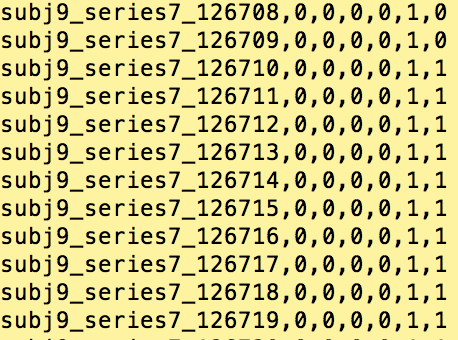
\includegraphics[height=1.3in]{multiLabel.png}
\end{center}
\end{column}
\end{columns}

\end{frame}


\begin{frame}
\frametitle{Evaluation Criteria}
\begin{columns}[T]
\begin{column}{.5\textwidth}
Mean Column-wise Area Under the Curve (MCAUC): the mean of individual areas under the ROC curve for each predicted columns.

\end{column}
\begin{column}{.5\textwidth}
\begin{center}
Sample ROC curve 
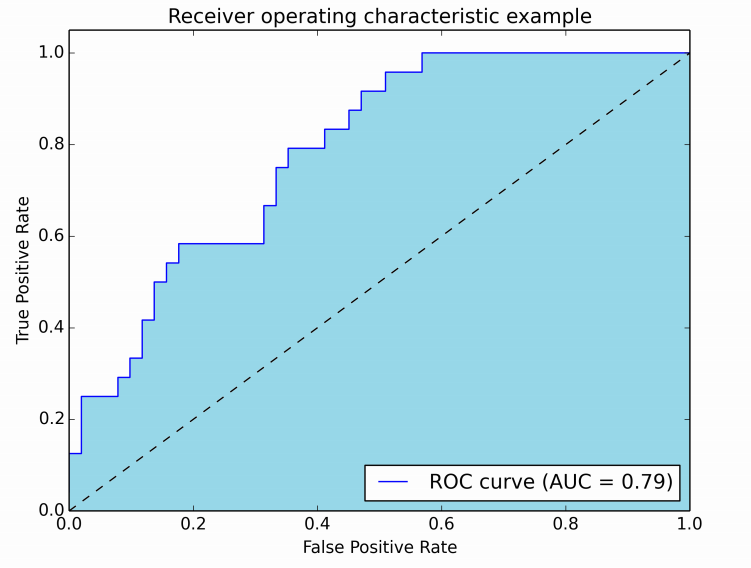
\includegraphics[height=1.5in]{9NpXJ.png}
\end{center}
\end{column}
\end{columns}


\end{frame}



\begin{frame}


\frametitle{Pipeline}
\begin{columns}[T]
\begin{column}{.1\textwidth}

\end{column}
\begin{column}{.8\textwidth}
\begin{block}{Preprocessing}
KDawn Filter: with hyper parameter 2-3-4 
\end{block}

\begin{block}{VLAD}
Number of clusters: $2^3\rightarrow 2^{15}$ 
\end{block}

\begin{block}{PCA}
number of components $=0.9$
\end{block}

\begin{block}{SVM - Linear \& Gaussian}
$C$ and $\gamma$ varies from $2^{-3}$ to $ 2^{3}$ 
\end{block}
\end{column} 
\begin{column}{.1\textwidth}

\end{column}
\end{columns}
\end{frame}


\begin{frame}
\frametitle{Performance optimization}
\begin{itemize}
\item Preprocess:  store the data for each component and use that in the next step of the pipeline
\item VLAD: save intermediate states as bumpy binary files and use them for the other parts of the pipeline
%save the cluster centroids in an instance variable (in kmeans algorithm) and reuse them in VLAD
\item kmeans: inertia convergence criteria. 
\end{itemize} 
\end{frame}



\begin{frame}
\frametitle{Pipeline Time}
Total time $ \sim   5h$ 
\begin{itemize}
\item Preprocessing: $< 1h$
\item All other steps:  $\sim4h$ 
\end{itemize}
VLAD:  $ \sim   12s$ with $32$ clusters and $1M$ local descriptors (with ubuntu dual core cpu, 3Gb ram)
\end{frame}








\begin{frame}
\frametitle{Table}
\begin{table}
\begin{tabular}{l l l}
\toprule
$\gamma$ & \textbf{C} & \textbf{mean score} \\

%\textbf{ SVM C} & \textbf{VLAD clusters} & \textbf{score} \\
%\midrule
%0.1 & 32 & 0.267\\
%1 & 32 & 0.268\\
%10 & 32 & 0.269\\

1 &1 & 0.36215\\
2 & 1 & 0.3222\\
4 & 1 & 0.27447\\
0.25&2&0.41857\\
%0.302951388889,0.5,2
%0.254340277778,1,2
%0.217881944444,2,2
%0.175347222222,4,2
\bottomrule
\end{tabular}
\caption{N components=3, $k=1024$}
\end{table}
\end{frame}


\begin{frame}
Number of clusters: $k=1024$: 
\frametitle{AUC}
\begin{center}
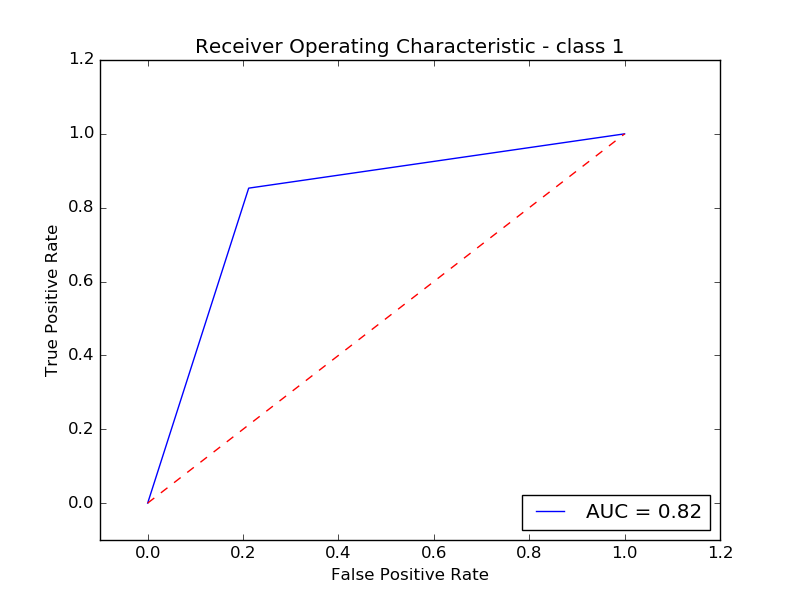
\includegraphics[height=3.0in]{roc.png}
\end{center}
\end{frame}


\begin{frame}
\frametitle{Obstacles}
\begin{itemize}
\item Domain knowledge.
\item Preprocessing steps
\item Implementing vlad that is compatible with scikit learn's pipeline.
\item Brutal HPC clusters.
\end{itemize}
\end{frame} 


\begin{frame}
\frametitle{Future work}
\begin{itemize}
\item Preprocess using filterbank which helps pick up low frequency but important features.
\item Training multiple models for the same problem.
\item No future data rule.
\end{itemize}
\end{frame} 


\begin{frame}
\frametitle{References}
\begin{itemize}
\item \url{https://www.kaggle.com/c/grasp-and-lift-eeg-detection/forums}
\item \url{https://github.com/alexandrebarachant/Grasp-and-lift-EEG-challenge}
\item \url{http://www.gipsa-lab.grenoble-inp.fr/~bertrand.rivet/references/Rivet2009a.pdf}
\item \url{https://lear.inrialpes.fr/pubs/2010/JDSP10/jegou_compactimagerepresentation.pdf}
\item \url{http://www.eecs.tufts.edu/~dsculley/papers/fastkmeans.pdf}

\end{itemize}
\end{frame} 


\begin{frame}
\frametitle{Acknowledgements}
\begin{itemize}
\item Zaid Harchaoui
\item Alexandre Barachant and Rafal Cyco\'n
\end{itemize}
\end{frame} 
%svm__C, myown__num_clusters,mean_validation_score,cv_validation_scores
%0.1, 32, 0.267913510101,  0.26278409  0.28858902  0.25236742
%1, 32, 0.268386994949,  0.26420455  0.29024621  0.25071023
%10, 32, 0.268702651515,  0.26420455  0.29048295  0.25142045
%100, 32, 0.269097222222,  0.26467803  0.29095644  0.2516572 

\begin{frame}
\Huge{\centerline{The End}}
\end{frame}



\end{document} 